\section{引言}
在近几年内深度卷积神经网络为图像分类领域带来了重大突破. 卷积神经网络最重要的两个特性是局部连接和权值共享. 因此, 和标准的前馈神经网络相比, 卷积神经网络具有非常少的连接和参数, 并且非常容易训练. 此外, 局部连接和权值共享分别满足了两个假设, 图像中距离近的像素之间的相关性远大于距离远的像素之间的相关性, 图像中的特征属性是和位置无关的. 

卷积神经网络中的卷积层利用卷积核来从图像中提取特征, 而卷积核就是需要训练的参数. 一般观点认为更深的网络可以从图像中提取出更高层次的更抽象的特征, 因而拥有更好的泛化能力. 但在实践当中使用深层的卷积神经网络时, 由于信号的逐层衰减, 输入信息不能有效地从网络浅层传递到深层. 同样地在误差反向传播阶段中, 误差梯度无法有效地从深层传递到浅层. 因此网络的深层和浅层部分的的训练速率不一致, 容易导致深层部分发生过拟合而浅层的部分却训练不充分, 这种现象被称为梯度弥散(gradient vanish)\cite{Glorot2010UnderstandingTD}.

基于归一化的方法, 例如Batch Normalization\cite{Ioffe2015BatchNA}, 可以有效解决梯度弥散问题, 提高深层神经网络的表现, 加速训练的收敛速度. 但随着网络的加深, 模型退化的现象依然发生. 有研究在卷积神经网络的基础上加入了``shortcut connections``结构, 提出了深度残差网络, 有效解决了网络过深导致模型退化的问题, 即使深达1000层的网络也能进行有效训练并收敛.

\section{卷积神经网络的图像分类应用}
在基于卷积神经网络的图像分类任务中, 模型通常是端对端(end-to-end)的, 即网络的输入就是图像本身或经过预处理的图像, 而输出就是图像属于各个类别的概率. 在这样的任务当中, 我们并不需要手工地设计特定的规则和特征提取器, 而是直接将图像以及标记类别的标签输入到网络中, 通过训练网络来得分类器. 经过端对端的训练后, 网络本身就包含了特征提取器和分类器.

在图像$\boldsymbol{x}$可能属于$K$个类别的分类任务当中, 用于分类预测的卷积神经网络$f$可以表达为
\begin{equation}
    \boldsymbol{y} = f(\boldsymbol{x}; \boldsymbol{\Theta}) \label{predict}
\end{equation}
其中图像$\boldsymbol{x}$是一个形状为$(\text{height}\times \text{width}\times \text{channels})$的三阶张量, height和width分别表示图像的行数和列数, channels表示图像的颜色通道数, 例如RGB图片有3个颜色通道. 卷积神经网络的输出值$\boldsymbol{y}$是$K$维的概率向量, 其第$k$个元素$y_k$表示预测得图像$\boldsymbol{x}$属于第$k$类的概率$p(\boldsymbol{x} \in \mathcal{C}_k ; \boldsymbol{\Theta})$. $\boldsymbol{\Theta}$表示卷积神经网络中所有可训练的参数, 包括权值和偏置等. 

在预测得到$\boldsymbol{x}$的类别概率向量$\boldsymbol{y}$后, 求得
\begin{equation}
    j = \arg \max_k y_k,
\end{equation}
之后, 我们把$\boldsymbol{x}$分到$\mathcal{C}_j$类中.


\subsection{网络参数的最大似然估计}
为了方便表示, 我们用one-hot编码的类别向量$\boldsymbol{t} = (t_1, \dots, t_K)^T$来表示图像$\boldsymbol{x}$所属类别, 满足
\begin{equation}
    t_k = 1\{\boldsymbol{x} \in \mathcal{C}_k\}
\end{equation}
其中$1\{\cdot\}$为指示函数, $1\{True\} = 1, 1\{False\}=0$.

对于图像$\boldsymbol{x}$, 我们利用式(\ref{predict})预测它属于各个类别的概率$\boldsymbol{y}$, 在这个基础上$\boldsymbol{x} \in \mathcal{C}_k$的条件概率为
\begin{equation}
    p(\boldsymbol{x} \in \mathcal{C}_k | \boldsymbol{x} ; \boldsymbol{\Theta}) = y_k, \quad k = 1, \dots, K
\end{equation}
由于
\begin{equation}
p(\boldsymbol{x} \in \mathcal{C}_k | \boldsymbol{x} ; \boldsymbol{\Theta}) = p(t_k = 1 | \boldsymbol{x} ; \boldsymbol{\Theta})
\end{equation}
类别向量$\boldsymbol{t}$的条件分布为
\begin{equation}
    p(\boldsymbol{t} | \boldsymbol{x} ; \boldsymbol{\Theta}) = \prod_{k=1}^K y_k^{t_k}
\end{equation}

对于一组已知类别的图像数据$D = \{(\boldsymbol{x_1}, \boldsymbol{t_1}), \dots, (\boldsymbol{x_M}, \boldsymbol{t_N})\}$, $\boldsymbol{x}$为图像, $\boldsymbol{t}$为类别标签. 我们希望用这些数据来训练网络, 可以直接写出似然函数
\begin{equation}
    \begin{aligned}
        \mathcal{L}(\boldsymbol{\Theta} | D) &= \prod_{m=1}^M p(\boldsymbol{t_m} | \boldsymbol{x_m} ; \boldsymbol{\theta})\\
        &= \prod_{m=1}^M \prod_{k=1}^K y_{mk}^{t_{mk}}
    \end{aligned}
\end{equation}
取似然函数的负对数
\begin{equation}
    -\log L(\boldsymbol{\Theta} | D) = -\sum_{m=1}^M \sum_{k=1}^K t_{mk} \log y_{mk}
\end{equation}
我们得到被称为交叉熵的损失函数
\begin{equation}
    E(\boldsymbol{\Theta} | D) = -\sum_{m=1}^M \sum_{k=1}^K t_{mk} \log y_{mk}
\end{equation}
最大化似然函数等价于最小化交叉熵损失函数, 网络的训练目的就是通过最小化交叉熵损失函数来求解网络的所有可训练参数$\boldsymbol{\Theta}$
\begin{equation}
    \hat{\boldsymbol{\Theta}} = \arg \min_{\Theta} E(\boldsymbol{\Theta} | D).
\end{equation}

参数是通过基于梯度的优化方法来迭代求解的, 最常见的方法是梯度下降. 每次的迭代将依次进行以下三个步骤
\begin{itemize}
    \item 前向传播, 利用当前的参数$\boldsymbol{\Theta}$和数据计算交叉熵损失函数
        \begin{equation*}
            E(\boldsymbol{\Theta}|D)
        \end{equation*}
    \item 反向传播, 计算损失函数关于所有可训练参数$\boldsymbol{\Theta}$的梯度
        \begin{equation*}
            \frac{\partial E(\boldsymbol{\Theta} | D)}{\partial \boldsymbol{\Theta}}
        \end{equation*}
    \item 梯度下降, 利用预先设定的学习速率$\eta$来更新参数
        \begin{equation*}
            \boldsymbol{\Theta} := \boldsymbol{\Theta} - \eta \frac{\partial E(\boldsymbol{\Theta} | D)}{\partial \boldsymbol{\Theta}}
        \end{equation*}
\end{itemize}
在适当的学习速率$\eta$下, 损失函数$E$总能收敛到某个局部极小值点. 实际我们并不需要求出全局最小值点, 因为这可能意味着模型过拟合.

\subsection{卷积神经网络}
到目前为止, 我们已经建立了模型的优化框架, 但并没有设计一个具体预测函数$f$, 即卷积神经网络. 网络的结构不是唯一的, 可以根据需要来设计. 一个卷积神经网络是由不同结构的模块串联而成的, 一般包含卷积层, 降采样(池化)层, Batch Normalization, 激活函数, 输出层等

一个图像的特征信息在网络中有两种格式, 第一种格式是特征图(feature maps), 是形状为$(\text{height}\times \text{width} \times \text{channels})$的三阶张量, 每个channel就是一个特征图. 第二种格式是特征向量(feature vector), 是一个向量, 向量的长度就是特征的维数. 特征图一般出现在卷积层和池化层, 特征向量一般出现在全连接层.

\subsubsection{卷积层}
描述图像的卷积层的时候, 我们需要先引入2维的离散卷积$*$. 设$f, h$分别是数字图像和卷积核, 定义$g = f * h$, 则图$g$在坐标$(x, y)$处的像素值为
\begin{equation}
    g(x, y) = \sum_{m=0}^{M-1} \sum_{n=0}^{N-1} f(m, n) h(x - m, y - n)
\end{equation}

现在考虑卷积神经网络中的卷积层$l$. , 则$l$层中的每个特征图$\boldsymbol{X}_j^l$是由卷积核$\boldsymbol{k}_{ji}^l$对前一层的各个特征图$\boldsymbol{X}_i^{l-1}$卷积再加上偏置项$b_j^l$得到的
\begin{equation}
    \boldsymbol{X}_j^l = \sum_{i=1}^{D_{l-1}} \boldsymbol{X}_i^{l-1} * \boldsymbol{k}_{ji}^l + b_j^l, \quad j = 1, \dots, D_l
\end{equation}
其中卷积核$\boldsymbol{k}$和偏置项$b$为可训练的参数. 第$l-1$层和$l$层分别有$D_{l-1}$和$D_l$个特征图, 这是由超参数控制的. 此外, 卷积运算$*$还有多种变体, 此处不展开描述.


\subsubsection{降采样层}
降采样层也称为池化层, 其作用是在尽可能保留特征信息的前提下减小特征图的尺寸, 从而较少网络的运算量, 提高特征的抽象性. 降采样层的每个特征图对应前一层的一个特征图, 降采样层的每个单元从前一层相应特征图中的一个对应的接收区域中计算采样值.  采样的方式包含最大采样, 平均采样和按概率采样, 前两种是最常见的. 接收区域也称为采样窗. 相邻采样窗的间隔称为采样步长. 采样层中特征图的计算可以表示为
\begin{equation}
    \boldsymbol{X}_j^l = down(\boldsymbol{X_j}^{l-1}), \quad j = 1, \dots, D_{l-1}
\end{equation}
\begin{figure}[!htbp]
\centering
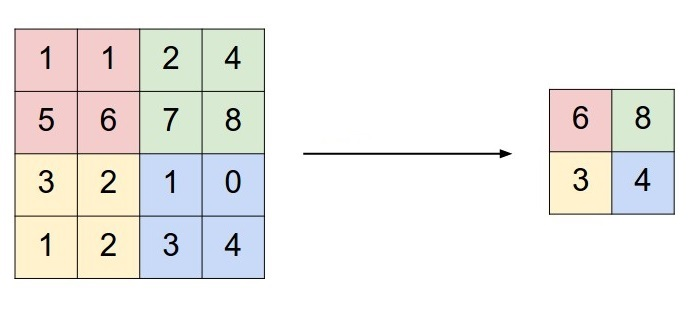
\includegraphics[width=12cm]{maxpool.jpeg}
\caption{最大采样, 采样窗大小为$2\times2$, 采样步长为$2\times2$.}
\label{maxpool} 
\end{figure}

\subsubsection{全连接层}
全连接层$l$的每个单元与前一层的所有单元是完全连接的, 这和普通的前馈神经网络是一致的. 表示为
\begin{equation}
    x_j^l = \sum_{i=1}^{D_{l-1}} w_{ji}^l x_i^{l-1} + b_j, \quad j = 1, \dots, D_l
\end{equation}



\subsubsection{激活函数}
激活函数层$l$的作用是对前一层的每个单元进行非线性变换, 这个变换被称为激活函数$g$. 为了方便表示, 我们把激活函数$g$扩展为向量形式
\begin{equation}
    g(
    \begin{pmatrix}
        x_{11} & \dots & x_{1n}\\
        \vdots & & \vdots\\
        x_{m1} & \dots & x_{mn}
    \end{pmatrix}
    )
    =
    \begin{pmatrix}
        g(x_{11}) & \dots & g(x_{1n})\\
        \vdots & & \vdots\\
        g(x_{m1}) & \dots & g(x_{mn})
    \end{pmatrix}.
\end{equation}
激活函数层对前一层的特征图的激活可以表示为
\begin{equation}
    \boldsymbol{X}_j^l = g(\boldsymbol{X}_j^{l-1}), \quad j = 1, \dots, D_{l-1}
\end{equation}
常见的激活函数有
\begin{align}
    ReLu(x) &= \max(0, x)\\
    tanh(x) &= \frac{e^x - e^{-x}}{e^x + e^{-x}}\\
    sigmoid(x) &= \frac{1}{1 + e^{-x}}
\end{align}
其中Rectified Linear Units(ReLu)是深度学习领域中最常用的激活函数, 因为它不会饱和, 当输入值大于0时, 导函数始终为1, 这不仅能有效缓解梯度弥散问题, 而且能加速训练的收敛.

\subsubsection{输出层}
在分类任务中, 假设类别数量为$K$, 通常会在卷积神经网络的最后一层$L$设置为含有$K$个单元的全连接层, 每个单元的输出值$x_j^L, j=1, \dots, K$表示相应类别的得分, 得分的相对大小反应了图像属于各个类别的可能性. 通常我们在最后的这层加入一个softmax函数, 将全连接层的$K$个输出值转换为概率值
\begin{equation}
    y_j = \frac{e^{x_j^L}}{\sum_{k=1}^K e^{x_k^L}}, \quad j = 1, \dots, K,
\end{equation}
向量化的表示为
\begin{equation}
    \boldsymbol{y} = \frac{1}{\sum_{k=1}^K e^{x_k^L}}
    \begin{pmatrix}
        e^{x_1^L}\\
        \vdots\\
        e^{x_K^L}
    \end{pmatrix}
\end{equation}
概率向量$\boldsymbol{y}$就是网络的输出值.

除了上述的模块, 本文不再对Batch Normalization, Locally connected等模块作描述. 一个卷积神经网络就由这些模块按照一定的顺序串联得到的. 图\ref{lenet}是LeNet5\cite{Lecun1998GradientbasedLA}的结构示意图. 可以看到, 卷积神经网络将原始图像的像素值逐层地进行变换, 最终得到类别的概率值.
\begin{figure}[!htbp]
\centering
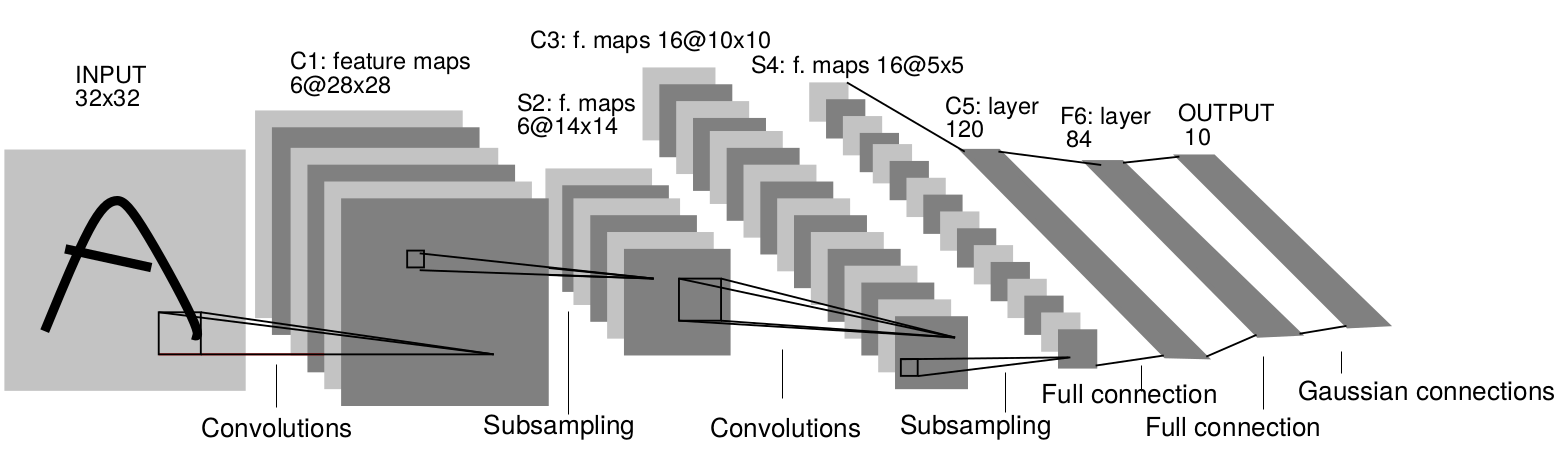
\includegraphics[width=17cm]{lenet.png}
\caption{用于手写数字分类卷积神经网络LeNet5的结构示意图.}
\label{lenet} 
\end{figure}

\subsection{残差网络}
我们知道, 典型卷积神经网络通常是多个模块按照一定的顺序串联起来的, 这样看起来就像一个扁平的网络, 代表有AlexNet和VGG\cite{Krizhevsky2012ImageNetCW,Simonyan2014VeryDC}. 图\ref{residual} (a)是这种扁平网络中的一部分. 深度残差网络\cite{He2016DeepRL,He2016IdentityMI}是在网络中特定位置加入了shortcut connection结构, 这可以让信号更容易地在网络中传播. 深度残差网络中的基本模块是残差单元, 其中卷积核的大小都是$3\times3$的. 图\ref{residual} (b)是残差单元的结构图, 一个深度残差网络可能包含数十上百个这样的残差单元. 一个残差单元的前向传播可以表示为
\begin{equation}
    \boldsymbol{Y} = \mathcal{F}(\boldsymbol{X}, \boldsymbol{W}) + \boldsymbol{X}
\end{equation}
其中$\mathcal{F}(\boldsymbol{X}, \boldsymbol{W})$表示信号$\boldsymbol{X}$沿着主路径传播的输出值, $\boldsymbol{W}$表示主路径中的权值参数. $\mathcal{F}(\boldsymbol{X}, \boldsymbol{W})$再加上捷径的信号$\boldsymbol{X}$, 就得到这个残差单元的输出信号$\boldsymbol{Y}$.

有时候残差单元的输入和输出的维数不一致, 例如特征图的尺寸或通道数不同. 这导致$\mathcal{F}(\boldsymbol{X}, \boldsymbol{W})$和$\boldsymbol{X}$不能直接相加. 当特征图尺寸不相同时, 可以在捷径中设置一个采样层来对$\boldsymbol{X}$进行采样, 从而调整捷径输出的特征图大小. 当特征图通道数不同的时候, 可以在捷径中设置一个$1\times1$的卷积层来对$\boldsymbol{X}$进行卷积, 从而改变捷径输出的特征图通道数, 可以表达为
\begin{equation}
  \boldsymbol{Y} = \mathcal{F}(\boldsymbol{X}, \boldsymbol{W}_1) + h(\boldsymbol{X}, \boldsymbol{W}_2)
\end{equation}

\begin{figure}[!htbp]
\centering
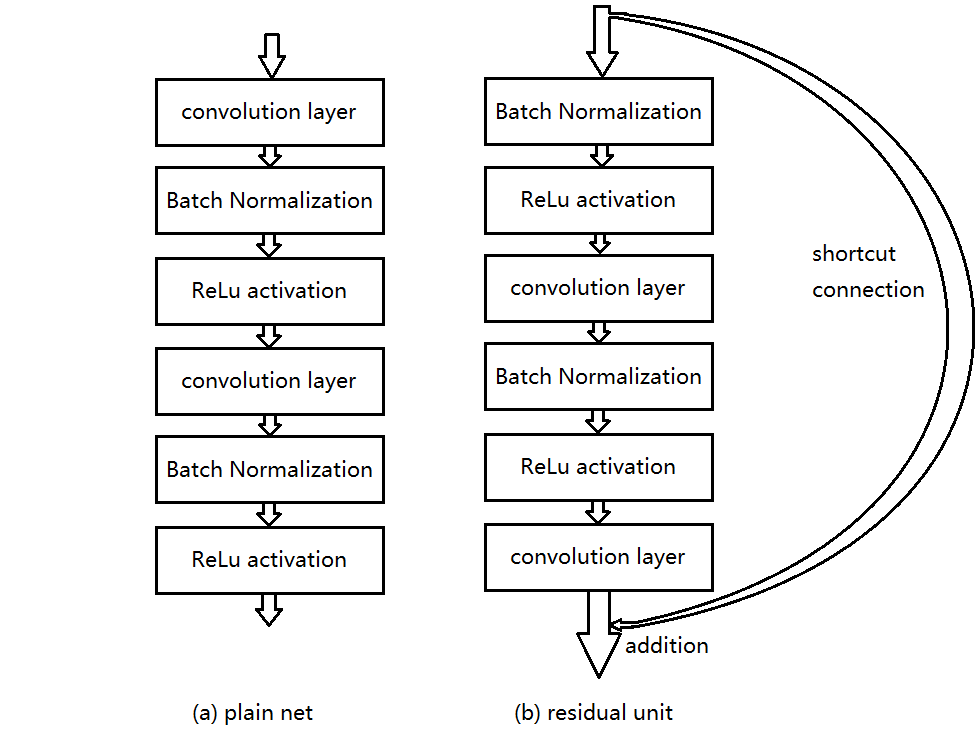
\includegraphics[width=12cm]{residual.png}
\caption{(a)是典型的卷积神经网络中的一部分, 信号从浅层到深层逐层传播. (b)是一个残差单元, 信号沿着主路径逐层传播的同时还会通过捷径传播. 深度残差网络通常可以包含数十上百个这样的残差单元.}
\label{residual} 
\end{figure}


\section{实验}
\subsection{CIFAR-10图像数据集}
我们的实验是在CIFAR-10图像数据集\cite{Krizhevsky2009LearningML}上进行, 这个数据集包含50,000张用于训练的图片和10,000张用于测试的图片. 每张图片为$32\times32\times3$的RGB格式彩色图片, 并且属于十个类别中的一类. 在搭建用于分类的深度残差网络后, 我们训练数据来训练网络的参数, 然后用测试数据来测试网络的准确率.

\subsection{网络结构和训练策略}
网络依次由1个卷积层和15个残差单元, 其中每5个残差单元构成一组, 3组单元输出的特征图的形状分别为$(32\times32\times16)$, $(16\times16\times32)$和$(8\times8\times64)$, 随后是一个全局平均池化层(global average pooling)\cite{Lin2013NetworkIN}, 然后是一层10个单元的全连接层, 最后添加了一个softmax函数作为输出. 详细的结构见图\ref{resnet}. 此外需要注意的是, 网络的第一个残差单元中, 在捷径的路径上还设置了一个Batch Normalization层和ReLu层.


\begin{figure}[!htbp]
\centering
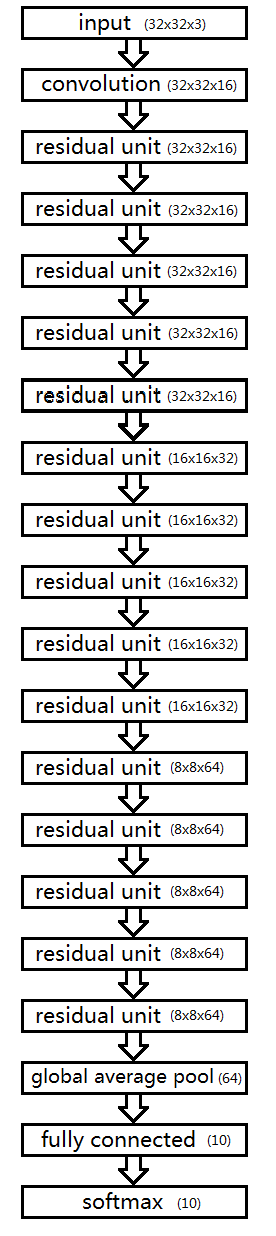
\includegraphics[width=4cm]{resnet.png}
\caption{本文中采用的网络的结构图. 在第一个残差单元中, 在捷径的路径上还设置了一个Batch Normalization层和ReLu层.}
\label{resnet} 
\end{figure}

在训练阶段中, 首先使用\cite{He2015DelvingDI}中的方法来初始化网络参数. 每次迭代的batch-size为128, 采用系数为0.9的Momentum梯度优化. $L2$正则化系数为0.0001. 在前500次迭代的时候使用0.01的学习速率来进行预热, 随后将学习速率调高到0.1. 当训练达到第32,000和48,000和64,000次迭代的时候将学习速率除以10. 训练在第80,000次迭代后停止. 数据增加的具体操作是, 在图像四周分别补上4个像素宽度的0像素, 使图像的形状变为$(36\times36\times3)$, 然后随机裁剪成$(32\times32\times3)$, 再经过$50\%$概率的水平翻转后就得到增加后的图像. 由于像素的取值范围是0至255, 这里的预处理方法是将每个像素乘以2后除以255, 最后再减去1, 这使得预处理后像素值的取值范围是 -1至1.

在测试阶段中, 不需要对数据进行补零和随机裁剪, 但需要进行相同的归一化预处理.

\subsection{结果}
使用Intel i5 - 7200u cpu和NVIDIA GeForce 940mx gpu进行计算, 训练经过20小时后达到迭代次数上限. 最后交叉熵损失函数值约为0.015. 网络在测试数据上的预测准确率为$91.1\%$.
\begin{figure}[!htbp]
\centering
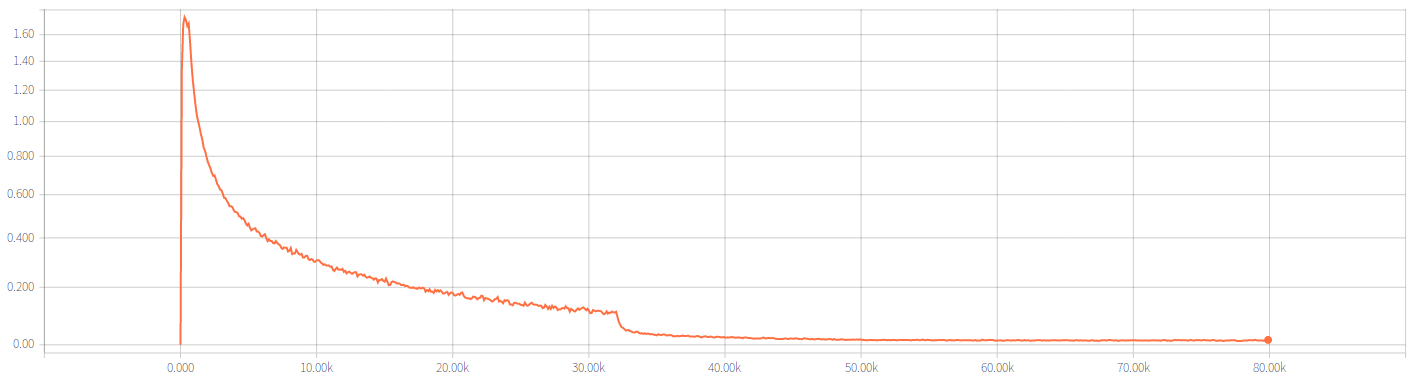
\includegraphics[width=17cm]{loss.png}
\caption{随着训练迭代次数增长, 交叉熵损失函数的变化曲线.}
\label{loss} 
\end{figure}


